\chapter{Tuning procedure and \textsc{mcnntunes}}
\label{chap:TuneprocedureCP5TuneandMCNNTUNES}

%The study of the underlying event, or more in general of soft QCD processes requires the use of Monte Carlo generators that often are based on phenomenological models with lots of free parameters. These free parameters must be tuned on experimental data in order to obtain meaningful results from the simulations. The procedure to estimate the best parameters values in order to best reproduce the observables under analysis is called \textit{tune}. 

As was introduced in the first chapter the tuning procedure can be really computational expensive, in fact it requires to run the generator a very large amount of times, and usually these MC generators are really expansive in terms of computational time required for just a single job.  
\\
To tune a certain number of parameters the number of Monte Carlo runs needed for the tuning procedure increases with the number of free parameters. In fact, the dimension of the parameter space increases with the number of the sampling we want to perform and the granularity we want to achieve. So, in the past, different approaches have been developed and used to tune these MC generators. A brief description is reported for each approach in the following list:
\begin{enumerate}[label=\arabic*)]
	\item \textbf{Manual tunes}: this approach is based on an optimization of the parameters made by eye. This is absolutely not the best way to tune some parameters, usually it requires a very large time for even semi-reasonable results since the process requires a very large number of iterations.   
	\item \textbf{Brute force tunes}: a better way would be to perform a very dense sampling in parameters space, run the generator with every configuration and then chose the configuration corresponding to the output that better describes the experimental data. This is very computationally expensive and a scan in a $5$ parameters space with $10$ divisions each requires $10^5=100000$ Monte Carlo runs this with a rising number of parameters becomes really impractical, also using computers batch systems as an example HTCondor.   
	\item \textbf{Parametrization-based tunes}: an even more better approach is to find a surrogate function to parameterize the response of the MC generator at different values of the parameters to tune, and try to study (minimize) this surrogate function instead of the real response of the generator. This is the current approach that is used in the high energy physics tune and that will be used in the following tunes presented in this thesis.
\end{enumerate}
This last approach will be discussed in more detail in the next section.

\section{Parametrization-based approach}

The parametrization-based approach is the most used method. The current state-of-art in the tuning procedure is to use a polynomial function to fit the response of the generator. Once the parametrization is performed the tuned parameters are given by the minimization of this parameterized response function. This approach based on the polynomial parametrization has been  implemented in the software \textsc{Professor} \cite{Buckley:2009bj}. 
\\
So the first step in the procedure is to fit the response of the generator using a surrogate function simpler to study than the real one (e.g. Professor instead of the arbitrary complex real function uses a polynomial fitted to well describe the real function).
\begin{equation}
	h(p)\ \xrightarrow{\quad \text{parametrization}\quad }\ \overline{h}(p)\quad ,
\end{equation}
where $h(p)$ is the vector of the observables distribution bins from MC simulations that are a function of the parameters. In this phase, these functions that give the values of the bins at the variation of the parameter values have been substituted by the surrogate ones $\overline{h}(p)$.  
%where the real function has been substituted by the surrogate one. 
\\
After that, a \textit{loss function} $\mathcal{L}(\overline{h}(p),h_{\text{data}})$ is defined between the surrogate function and the experimental data. A common choice for it is the $\chi^2$ function defined as:
\begin{equation}
	\mathcal{L}(\overline{h}(p),h_{\text{data}})\equiv \chi^2=\frac{(\overline{h}(p)-h_{\text{data}})^2}{\sigma^2}\quad.
\end{equation}
where $\sigma^2$ is the vector of the experimental squared error on each bin.  
In the end, to find the best parameters estimation, this loss function needs to be minimized. The set of parameters $p_{\text{best}}$ is the best evaluation that our generator can provide for the real values and we are going to call this set of best parameters: \textit{tune}.
\begin{equation}
	p_{\text{best}}=\arg\,\min_p\ \mathcal{L}(\overline{h}(p),h_{\text{data}})\quad.
\end{equation}
In this thesis instead of the common software \textsc{professor} based on the polynomial parameterization, it is used the machine learning approach implemented in \textsc{mcnntunes} software \cite{MCNNTUNESonGitHub}
using Feed Forward Neural Networks. \textsc{mcnntunes} is a software developed by S. Carrazza, S. Alioli and M. Lazzarin presented in \cite{MCNNTUNESarticle} based on machine learning library TensorFlow \cite{tensorflow2015-whitepaper}. \textsc{mcnntunes} is written in Python and uses Feed Forward Neural Networks that are trained in order to learn the generator behaviour with respect to the parameter variations. This removes the polynomial constraint in the fit of the generator response function in fact one of the main features of the Neural Networks (NNs) is that they are universal function approximators.
\\
A brief introduction follows on machine learning and in particular on NNs in order to understand better how \textsc{mcnntunes} works.

\section{Machine Learning and Neural Networks}
  
Machine learning (ML) is a particular type of Artificial Intelligence and consists of the implementation of systems that learn automatically by the data that are fed into them and not by the explicit programming of the algorithm. It is clear that ML requires the training of the algorithm in order to have a predictive output related to the problem under analysis. The training is the most important step in the ML approach in fact is this step that gives to the ML the ability to return a predictive output; without it the output we get is not able to give us a meaningful result.
\\
A particular type of ML is Deep Learning which uses neural networks with more than one layer organized in a hierarchical structure to solve the problem. This is the type of ML we are interested in. But before we start with the explanation of the simple possible neural network that can be created in order to understand the basis in the logic of each unit that is going to compose the neural network. 


\subsection{Neural Networks - Perceptron}

The concept of the Neural Network (NN) was developed in 1958 by Frank Rosenblatt. He introduces the simpler example of NN: the perceptron \cite{Perceptron}. A representation of a percepton is shown in \figRef{fig:Perceptron} the input values are weighted and summed, an additional offset $b$ can be introduced, and then the weighted-sum is passed to an activation function (step function). So, the output that the perceptron returns is:
\begin{equation}
	h(x)= \text{step}\bigg(\displaystyle\sum_j w^j\, x_j + b\bigg)
\end{equation}

\begin{figure}[!htb]
	\centering
	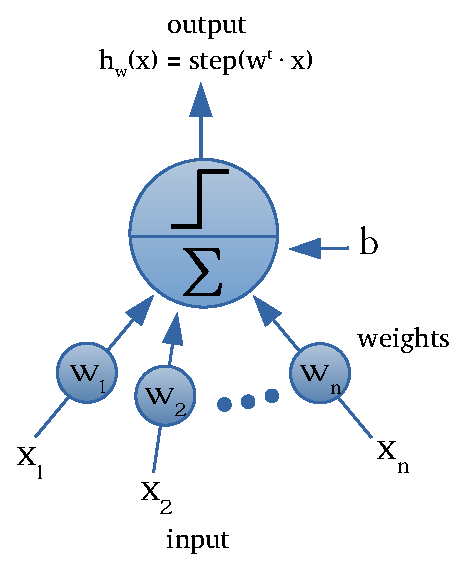
\includegraphics[scale=0.7]{{img/Perceptron2.pdf}}
	\caption{A schematic representation of a perceptron.}
	\label{fig:Perceptron}
\end{figure}

\noindent The revolutionary feature of the perceptron was the ability of learning by an adjustment of the weights. Anyway, a single perceptron is not enough since these kinds of logical units have lots of limitations. An example of a limitation for the perceptron is shown in \figRef{fig:XORproblem} where the impossibility of implementing a \textsc{xor} operation using a perceptron is shown with a graphical explanation. The perceptron is a linear classification algorithm and in the image is represented as a blue line that set a boundary for the acceptation of the hypothesis.

\begin{figure}[!htb]
	\centering
	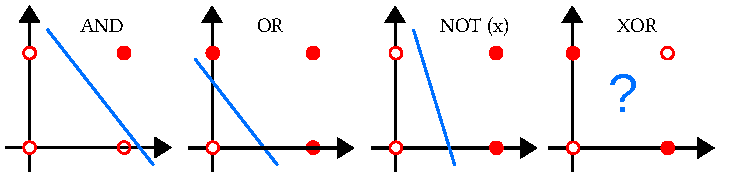
\includegraphics[width=14cm]{{img/XORproblem.pdf}}
	\caption{The figure shows one of the limitations of the perceptron. The \textsc{xor} operation is not possible with a linear cut. In the figure the two axes are related to the two boolean variables $x$ and $y$; the possible values for these variables are only $0$ and $1$, the four combinations are indicated by the red circles: $(0,0)$, $(1,0)$, $(0,1)$ and $(1,1)$. The first image shows the \textsc{and} operation the full red circle indicates the accepted point $(1,1)$, the discrimination can be performed correctly with just one straight line (perceptron discrimination). Also, the \textsc{or} ($(0,1)$, $(1,0)$, $(1,1)$) and the \textsc{not x} ($(0,0)$, $(0,1)$) ones can be implemented correctly using perceptron. But this cannot be done for the \textsc{xor} operation ($(0,1)$, $(1,0)$).}
	\label{fig:XORproblem}
\end{figure}

To describe more complex problems it has to be introduced the concept of NN with more than one unit if we want to eliminate these limitations and approximate every type of function.

\subsection{Feed-Forward Neural Networks}

In a Neural Network different units called "neurons" are linked together. Different types of NNs exist and they are classified according to the various ways the neurons are linked to each other. We are interested in \textit{fully-connected Feed-Forward NNs}, which are the ones used in \textsc{mcnntunes}. 
\\
In fully-connected NNs each neuron from a layer is connected to every neuron in the next layer, while the Feed Forward attribute refers to the fact that the NN have no internal recursions (loops) between neurons but all the neurons from a layer are connected forward to the ones of the next layer.
\\
\figRef{fig:NNesample} shows a schematic view of a fully-connected feed-forward multi-layer NN. The basic idea is that the neurons can get some value in input and return a value as output. The output of a neuron is then sent to all the neurons in the next layer and weighted differently for each one. 
To be more specific: each unit $j$ in the hidden layer $(i)$ takes a vector of values $x^k$, that come from all the $k$ neurons of the previous layer, and an offset $\vartheta_j$ as input, computes the weighted sum $\sum_k w_{kj}x^k$ and apply the activation function $\phi$ to the result. Common choices for this function are \textit{tanh} or \textit{sigmoid} functions. So, the total output of the $(i)$-th layer in the network is the function:
\begin{equation}
	f^{(i)}(x) = \displaystyle\sum_{j=1}^{N^{(i)}} \varphi \left( \displaystyle\sum_k w^{(i)}_{kj}x^k + \vartheta_j^{(i)} \right)\quad,
\end{equation}
where $N^{(i)}$ is the number of hidden units in the $(i)$-th layer. 
\\ 
One of the prominent features of the NNs is that they are universal function approximators \cite{HORNIK1991251, LESHNO1993861} the only request for this is that a sufficient number of hidden layers is available. This is the main reason why we want to use a NN based approach instead of the polynomial one implemented in \textsc{professor}.


\begin{figure}[!htb]
	\centering
	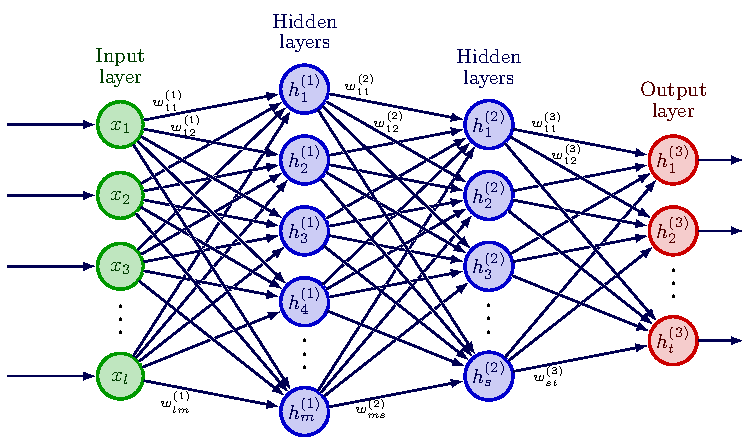
\includegraphics[width=0.95\textwidth]{{img/NN.pdf}}
	\caption{A fully-connected feed-forward neural network with more than one hidden layer, the green one is the input layer and takes the value in input and usually scale them in the range $[0,1]$ and then the data sequentially go trough the neurons in the hidden layers (blue) where all the steps described above are performed for each layer. At the end the results of the computation are collected by the output layer (red). }
	\label{fig:NNesample}
\end{figure}

\noindent As mentioned before the main feature of all the types of NNs is the ability to learn from data without being directly programmed.
But to this and so get some predictive results from the NN a learning algorithm has to be defined.
\\
A common training algorithm for the NN is the \textit{back-propagation}, where a set of Monte Carlo simulations is used to train the NN. The back-propagation procedure is based on the idea of changing the weights, $w_{jk}$, and the offsets, $\vartheta_{j}$, in order to minimize a loss function usually defined as the mean squared error ($E$):
\begin{equation}
	E=\frac{1}{2}\displaystyle\sum_i(h_{i}(x^j,w_{jk})-d_i)^2\quad,
\end{equation}  
where the $h_{i}$ are the value in output from the NN and the $d_{i}$ the real value known from the Monte Carlo truth.
\\
In the back-propagation algorithm the weight and the coefficients are updated using the \textit{steepest-descent minimization}:
\begin{equation}
	w_{jk}^{(i+1)}=w_{jk}^{(i)}-\lambda\left( \frac{\partial E}{\partial w_{jk}} \right)^{(i)}
	\quad; \ \qquad
	\vartheta_{j}^{(i+1)}=\vartheta_{j}^{(i)}-\lambda\left( \frac{\partial E}{\partial \vartheta_{j}} \right)^{(i)}
	\label{eq:learning_bp}
\end{equation}
where $\lambda$ is the \textit{learning rate} and is a user-tunable free parameter and it controls how much change the weights each time the weights are updated.
It is one of the main parameters in the neural networks a too small value for it can lead to a failure in the training procedure while a too large one can lead to unstable results. 
\\
The \textit{mini-batches} are subsets of our training set that contains the Monte Carlo simulations that are used to calculate the gradient. The size of the mini-batches used to train the NN is also a free parameter: smaller batches are faster to compute but the gradient direction is not the real one just an approximation; while a bigger batch size gives a good approximation of the direction of the steepest-descent but can be computationally expensive. 
\\
The number of evaluations of the entire training set is called \textit{epoch} and it is tunable by the user.
\\
Note that the batch size and the number of epochs are strictly related. A training set of 50 MC runs with a batch size of 10 and a number of epochs of 1000 requires 5000 iterations while if we use a batch size of 25 it requires only 2000 iterations to run over the whole training set.
\\
A schematic representation of the training process is displayed in \figRef{fig:training2} where the training set is subdivided into the mini-batches that one by one are fed to the NN. Then, the Monte Carlo truth and the output of the network are used to compute the loss function $E$, using this information the back-propagation, based on the gradient descend algorithm, updates the weights in the descent direction of the gradient calculated using the mini-batch. All the procedure is repeated with every mini-batch and for a user tunable number of epochs.

Note that the prediction capability of the Neural Network is dependent on the selection of all these user-tunable parameters that control the Neural Network architecture. All these parameters are usually referred to as \textit{hyperparameters}. 

\begin{figure}[!htb]
	\centering
	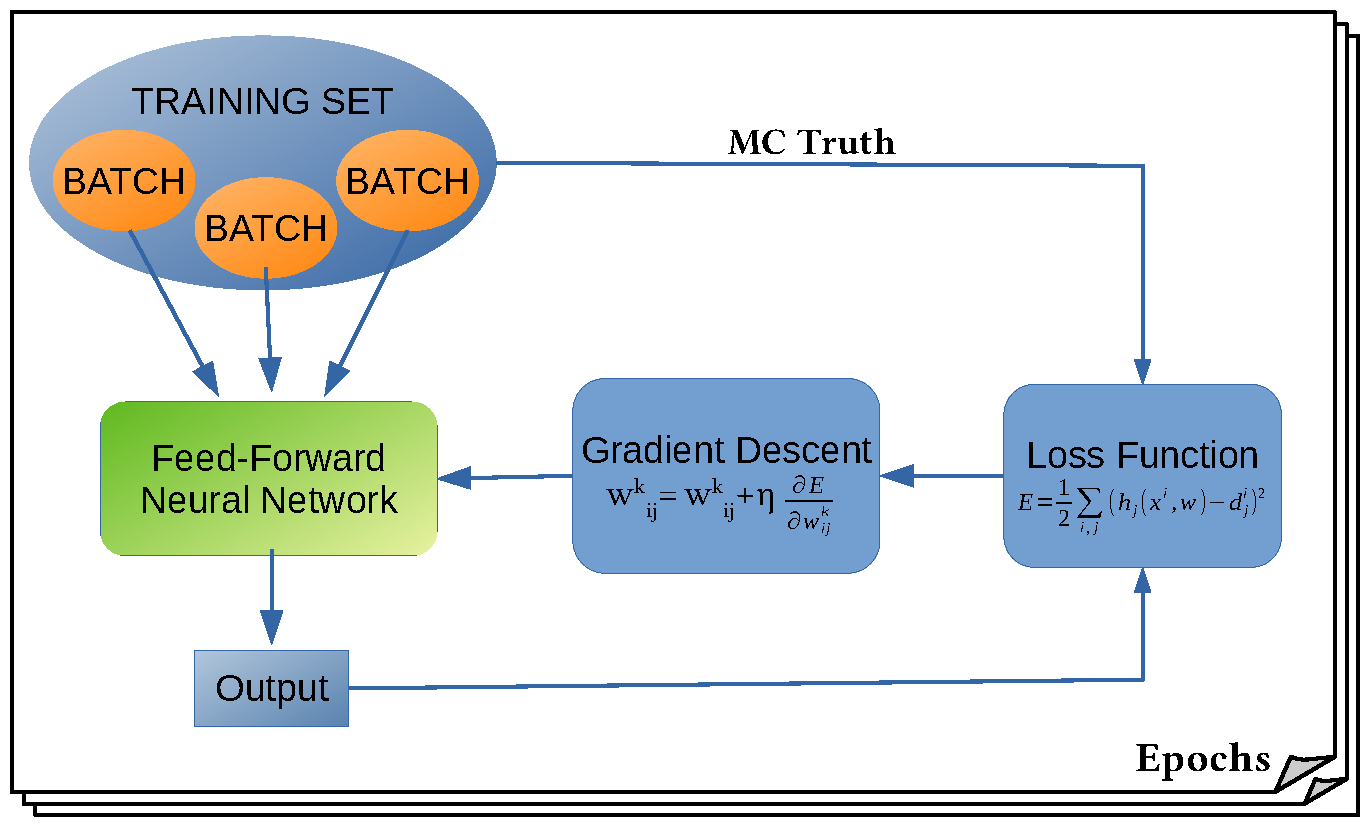
\includegraphics[width=14cm]{{img/Training2.pdf}}
	\caption{The training set used to train the NN is divided into mini-batch (the mini-batch size is a user tunable parameter) then one by one the batches are fed to the NN the output of the network together with the Monte Carlo truth are used to calculate the loss function. Then the weights and the offset are updated as described in \eqRef{eq:learning_bp} with the back-propagation algorithm. This is done with each mini-batch in the training set and for a number of epochs defined by the user. }
	\label{fig:training2}
\end{figure}


%%%%%%%\section{Previous Tune for the Underlying Event} OLD

In the next section, \texttt{mcnntunes} is introduced and all its working modes are explained in detail. 

\section{MCNNTUNES}

\textsc{mcnntunes} \cite{MCNNTUNESarticle} is a Shower Monte Carlo generators tuning tool that implements a tune procedure based on the use of Feed Forward Neural Networks. The advantage of using FFNNs has been described above and it is that they are universal function approximators at the simple cost of having a sufficient number of hidden units in the hidden layers. This feature allows us to remove the polynomial bias present in \textsc{professor} tool.
\\
\textsc{mcnntunes} offers two different main operation modes: \textit{PerBin Model} and \textit{Inverse Model}. The first one is based on an approach similar to the one in \textsc{professor} but where the response of the generator is parameterized using these FFNNs, one for each bin; the latter is a totally new approach where the NN (only one in this case) is trained to learn the inverse function of the generator response and then used to tries to infer the parameters value starting from the experimental values of the bins in the distributions used.
\\

\medskip

\subsection{Sampling Phase and Training Set Generation}

The two approaches have the same starting point that is a sampling of the parameter space (e.g. for the UE analysis we use the parameters space shown in \tableRef{table:CP5variations}), then the generator is run with every sampled configuration. 
All these MC runs are going to build our dataset which is called \textit{training set}.
\\
\figRef{fig:worksampling} shows a schematic explanation of how the sampling phase and the training set generation were performed using the CMS software environment referred as CMSSW. CMSSW is present on the public machine cluster of the \textsc{cern} called LXPLUS (LinuX Public Login User Service). 
In more detail the sampling starts by means of the  \textsc{mcnntunes} script called \textsc{mcnntemplate} with a sampling of the defined parameter space. The sampling generates  $N$ different configurations for the parameters to tune, these are then encapsulated in a runcard for \textsc{pythia} that contains all the necessary information to make \textsc{pythia} work properly (beams energies, type of event to simulate etc.). Once these runcard are saved the \textsc{pythia} generator is run with every configuration generated and this is performed not locally but on a computers batch (e.g. the \textsc{cern} one CondorHT) in order to gets all the results in few days. The runcards we pass to Condor contain also the information on the analysis we want to perform and on how to fill the various histograms for the observables. Once the generators runs end the outputs are saved in the \textsc{yoda} format \cite{YODA}, that is a standard type of data file for these analyses also used in Rivet. The set of these \textsc{yoda} files, containing the information on the MC runs, composes our training set that then can be used for the tuning procedure.

\begin{figure}[!htb]
	\centering
	\includegraphics[width=0.95\textwidth]{{img/Worksampling.pdf}}
	\caption{A schematic description of the main step from the sampling phase to the generation of the training set used for the tune procedure. These shows how the work was performed in CMSSW environment. The starting point and the final tune procedure are both controlled by \textsc{mcnntunes}. In the middle of these two phases the generation of the training set is required, this is performed running the generator many times.}
	\label{fig:worksampling}
\end{figure}

\medskip

\textsc{mcnntunes} offers also the possibility of changing the value of the hyperparameters. 
%The value that can be modified for the Neural Network. 
It is possible to choose the NN architecture: the number of hidden layers, the number of neurons for each layer and the activation function used. It is also possible to set the number of epochs, the batch size and the learning rate in order to have the best train for the architecture selected and other choices are possible. This is really important in order to get the best possible results for the tune. Below we are going to discuss the procedure used for the Inverse Model in order to search for the best hyperparameters configuration.

\subsection{PerBin Model}
\label{sec:PerBinModel}

PerBin Model is a parametrisation-based method. The main idea, as shown in \figRef{fig:PerBinModel_schematic} is to build a model (i.e. a neural network) for each bin in order to parameterize the generator output. Each NN takes the parameter values as input and returns the bin value as output.
\\
All these NNs are then trained feeding the MC runs from the training set and  using a gradient-based algorithm, as usual for feed forward neural networks, with mean squared errors as loss function.
\\
Once, the NN is trained, the last step is the tune in which one actually gets the best parameters estimation.  This step defines a surrogate loss function for the tuning problem. In fact, the parameterization step returns a model $h^{(i)}(\mathbf{p})$ for each bin, $i$, where $\mathbf{p}$ is the vector of the parameters. 
\\
Then, this surrogate loss function is defined as:
\begin{equation}
	\chi^2=\displaystyle\sum_{i=1}^N\frac{\left( h^{(i)}(\mathbf{p})-h_{exp}^{(i)}\right)^2}{\sigma_{(i)}^2}
\end{equation}
need to be minimized in order to evaluate the best estimation for the parameters. In \texttt{mcnntunes} this minimization is performed using the CMA-ES algorithm \cite{CMAES}.
\\
So the best estimation for the parameters is the configuration of parameters that minimizes this $\chi^2$.  

\begin{figure}[!htb]
	\centering
	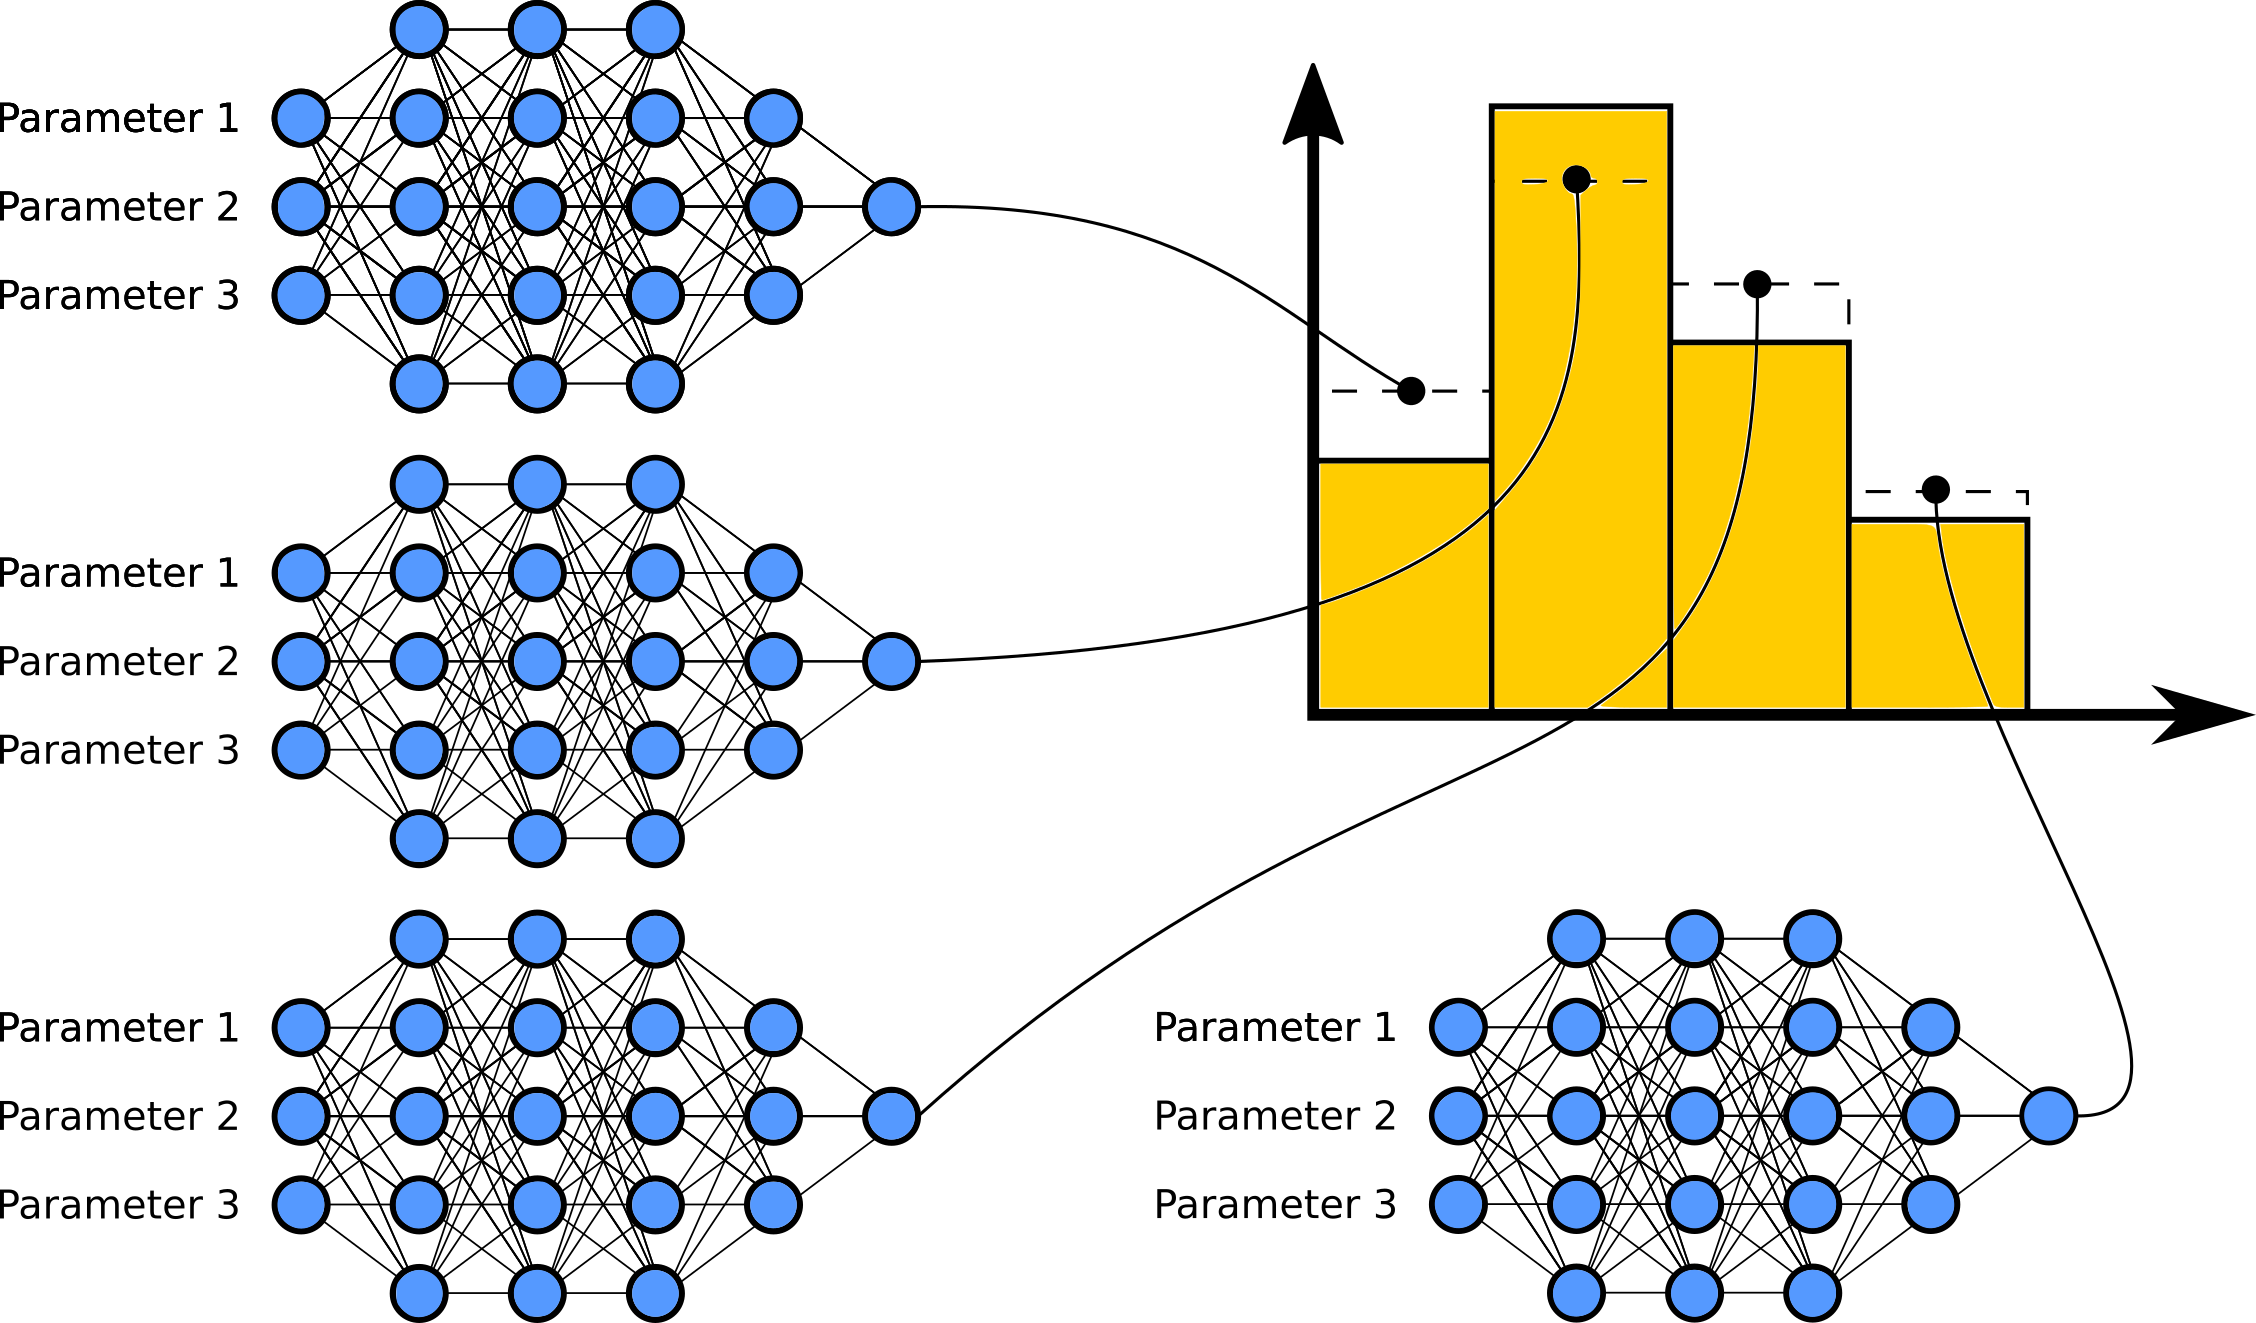
\includegraphics[width=0.8\textwidth]{{img/PerBinModel.png}}
	\caption{Figure from \cite{MCNNTUNESarticle}}
	\label{fig:PerBinModel_schematic}
\end{figure}

\subsubsection{Error evaluation}

\textsc{mcnntunes} PerBin model as introduced in \cite{MCNNTUNESarticle} did not have a proper error evaluation on the minimized parameters. In fact it was using as error the final width of the distribution of sampled point in the CMA-ES algorithm. But, this was not working the errors were underestimated on all the minimized parameters. Thanks to S. Carrazza and with the help of M. Lazzarin we had the opportunity of handle the code and add a proper error estimation.

Now, the error evaluation for the PerBin model is given by the definition of a confidence interval using the $\chi^2$ function.
In fact, as shown in section 9.6 and 9.7 of \cite{cowan}, for an estimators vector $\hat{h}(\mathbf{p})=(\hat{h}^{(1)}(\mathbf{p}),\hat{h}^{(2)}(\mathbf{p}),\dots,\hat{h}^{(n)}(\mathbf{p}))$ for the parameters $\mathbf{p}$ the probability distribution function and the likelihood (the $\chi^2$ in our case) in limit of a large set of estimators and so of degrees of freedom ($\nu$)\footnote{In other cases this is a good approximation.} is approximately Gaussian distributed with mean $\nu$ and variance $2\nu$. The probability distribution function for the estimators is then:
\begin{equation}
f(\hat{h}(\mathbf{p})|h(\mathbf{p})) = \frac{1}{(2\pi)^{n/2}|V|^{1/2}}\exp\left[ -\frac{1}{2}\left(\hat{h}(\mathbf{p}) - h(\mathbf{p})\right)^T V^{-1} \left(\hat{h}(\mathbf{p}) - h(\mathbf{p})\right) \right] \ ,
\end{equation}
where $T$ is the transposed vector and $V^{-1}$ is the inverse covariance matrix. 
%Can be shown that also the likelihood is Gaussian as the probability distribution function. 
%So a changing in the parameter give a calculable variation in the $\chi^2$
So, we can define our confidence interval using the $\chi^2$ statistic as: 
\begin{equation}
	\frac{\chi^2(\text{c.i.})}{N_{dof}}= \frac{\chi^2_{min}}{N_{dof}}+\frac{Q_\gamma}{N_{dof}}
	\label{eq:chi2_variation}
\end{equation} 
The variation is dependent on the number of parameters and on the chosen confidence level ($1\sigma=0.683$ in our case) and a list of the values is reported in \tableRef{table:percentile}.

\begin{table}
	\centering
	\begin{tabular}{c | c c c c c}
		\multirow{ 2}{*}{percentile} & \multicolumn{5}{c}{$Q_\gamma$}\\\cline{2-6}
		& $\nu=1$ & $\nu=2$ & $\nu=3$ & $\nu=4$ & $\nu=5$ \\\hline\hline
		$0.683$& $ 1.00 $ & $ 2.30 $ & $ 3.53 $ & $ 4.72 $ & $ 5.89 $ \\
		$0.90$ &  $ 2.71 $ & $ 4.61 $ & $ 6.25 $ & $ 7.82 $ & $ 9.24 $ \\
		$0.95$ & $ 3.84 $ & $ 5.99 $ & $ 7.82 $ & $ 9.49 $ & $ 11.1 $ \\
		$0.99$ & $ 6.63 $ & $ 9.21 $ & $ 11.3 $ & $ 13.3 $ & $ 15.1 $ \\
	\end{tabular}
	\caption{The table report the values of the quantile $Q_\gamma$ for different percentile and for different number of degree of freedom $\nu$. The row corresponding to $0.683$ ($1\sigma$) is the one of our interest.}
	\label{table:percentile}
\end{table}

\noindent Then, the error is defined as the value of the parameters that give a deviation from the minimum value of the $\chi^2/N_{dof}$ equal to the $Q_\gamma/N_{dof}$ value for a confidence level of $0.683$, as defined in \eqRef{eq:chi2_variation}.
\\
An example for the evaluation in \texttt{mcnntunes} is shown in \figRef{fig:exampleChi2Variation} where the green line is the deviation from the minimum value of the $\chi^2$ defined in \eqRef{eq:chi2_variation} and the errors are given by the points where the $\chi^2/DoF$ reaches these values, in the figure given by the intersection of the blue and the green line.

\begin{figure}[!htb]
	\centering
	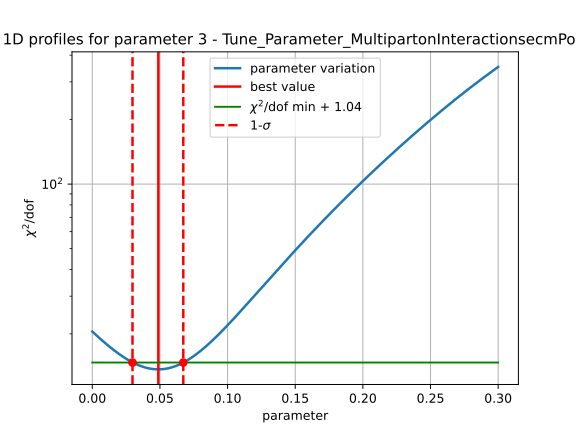
\includegraphics[width=0.6\textwidth]{{img/exampleChi2Variation.png}}
	\caption{This figure shows the error evaluation in \texttt{mcnntunes} for the \texttt{MultipartonInteractions:ecmPow} \texttt{Pythia8} parameter. The blue line is the value of the $\chi^2/N_{dof}$ evaluated for different parameter values. The best estimation is indicated by the vertical red line, while the green line is the quantity in \eqRef{eq:chi2_variation}. The error is evaluated from the intersection of blue and green lines.
	}
	\label{fig:exampleChi2Variation}
\end{figure}

\subsection{Negative aspects}

One of the negative aspects is that this model is more computationally expensive than the Inverse model discussed below. This is due to the large number of NNs built and trained from this model. 
The high cost in terms of time required to get the model work do not give the possibility for a scan in the hyperparameters space in order to obtain the best configuration for the NN architecture. 
\\
This can impose some limitations on the model performance that cannot get its maximum  performance.

\subsection{Inverse Model}

The Inverse Model is the most innovative tuning procedure introduced by \texttt{mcnntunes}. This model contrarily to the PerBin Model takes the bins of the histograms as input and returns parameter values as output. For the Inverse Model the NN used is only one as shown schematically in \figRef{fig:InverseModel_schematic}. What the Inverse Model tries to do is to learn the inverted model of the generator. So starting from the observed values the model tries to reproduce the parameters values necessary to get the histograms we use as input.
\\
The model is built and then trained with the training set introduced before. Once the model is trained feeding the experimental data to the NN this can try to infer the values of the parameters required to get the output. 

\begin{figure}[!htb]
	\centering
	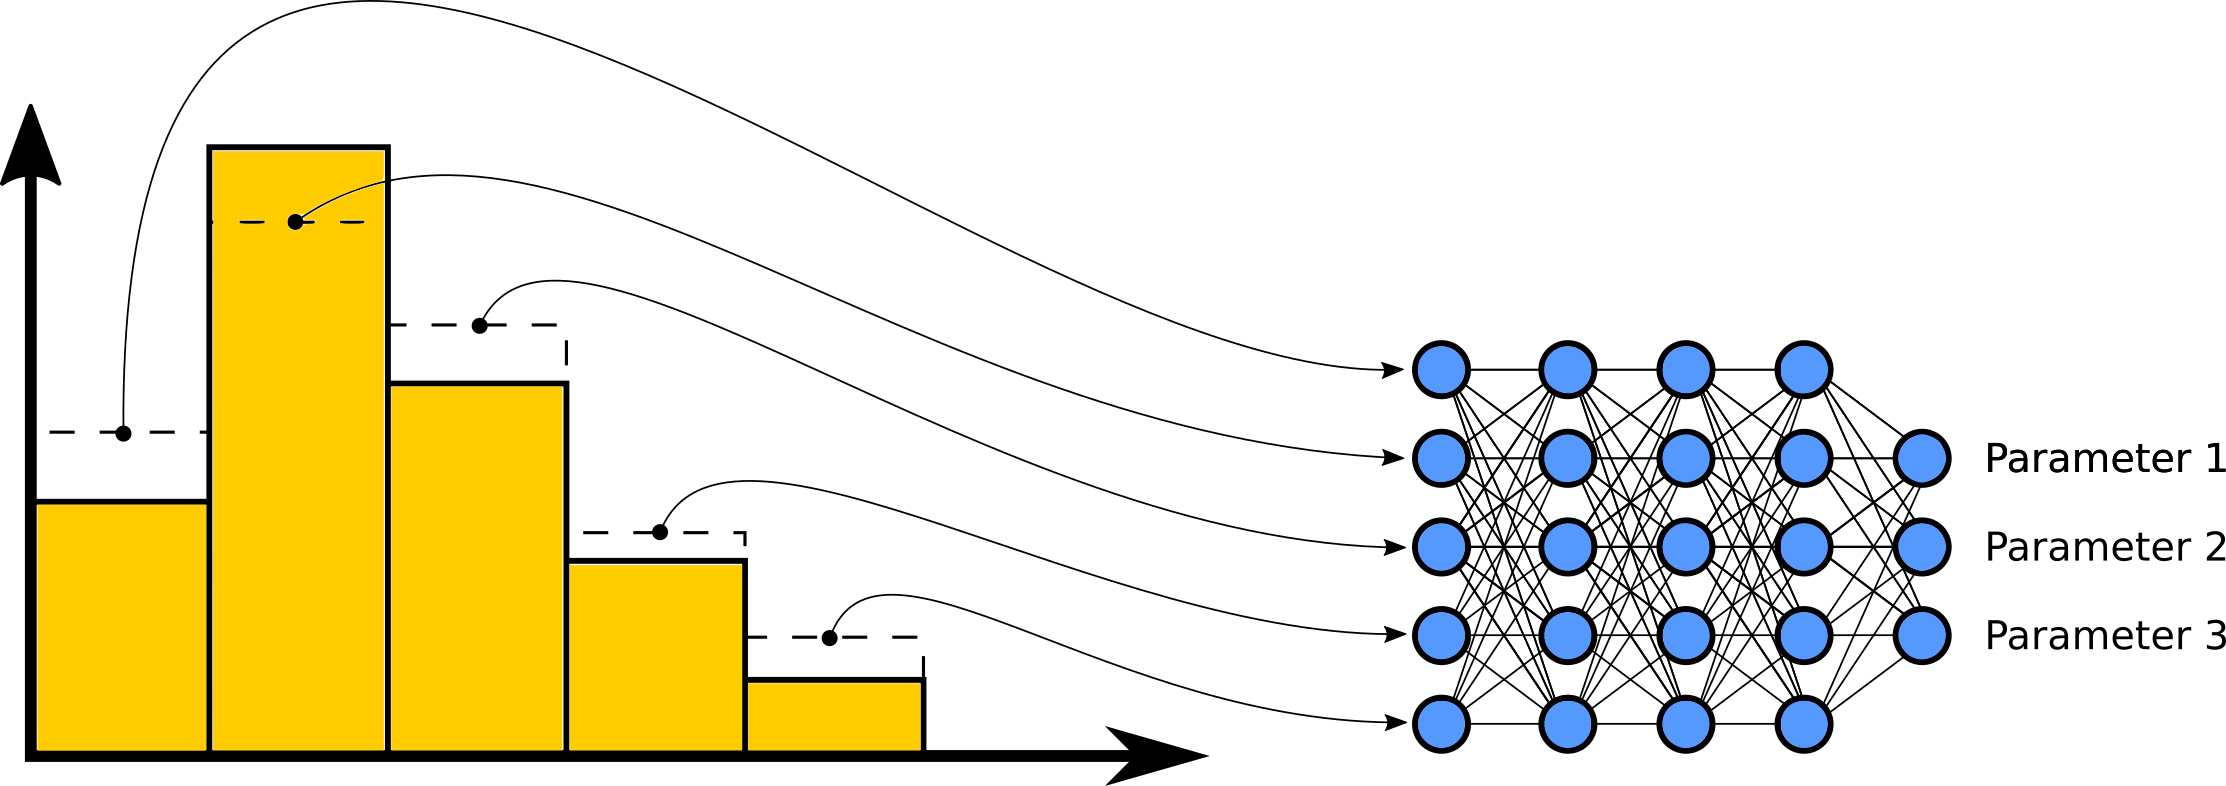
\includegraphics[width=0.8\textwidth]{{img/InverseModel.png}}
	\caption{Figure from \cite{MCNNTUNESarticle}}
	\label{fig:InverseModel_schematic}
\end{figure}

\subsubsection{Errors evaluation}

The errors are evaluated in a different way with respect to PerBin model. In fact, in the Inverse Model there is no a minimization step, and the error is evaluated by a re-sampling of the experimental data using a \textit{multivariate Gaussian Distribution}, as the one in \eqRef{eq:gaussianDristribution} with a diagonal covariance matrix that has experimental uncertainties on the main diagonal.
\begin{equation}
	f(x_i; h^{(i)}_{\text{exp}}, \sigma^{(i)}_{\text{exp}})\,=\,\mathcal{N}\cdot\exp\left[ 
	-\frac{1}{2}
	\displaystyle\sum_{j=1}^{N_{bins}}
	\frac{\left( 
	x_i - h^{(i)}_{\text{exp}} 
	\right)^2}{{\sigma^{(i)}_{\text{exp}}}^2} 
	\right]
	\label{eq:gaussianDristribution}
\end{equation}
So, a set of histograms is generated, then this is fed to the NN and a distribution of predictions is generated. An example is shown in \figRef{fig:InverseModel_predictionsSpread}, from this distribution one can compute the error by evaluating the standard deviation.

\begin{figure}[!htb]
	\centering
	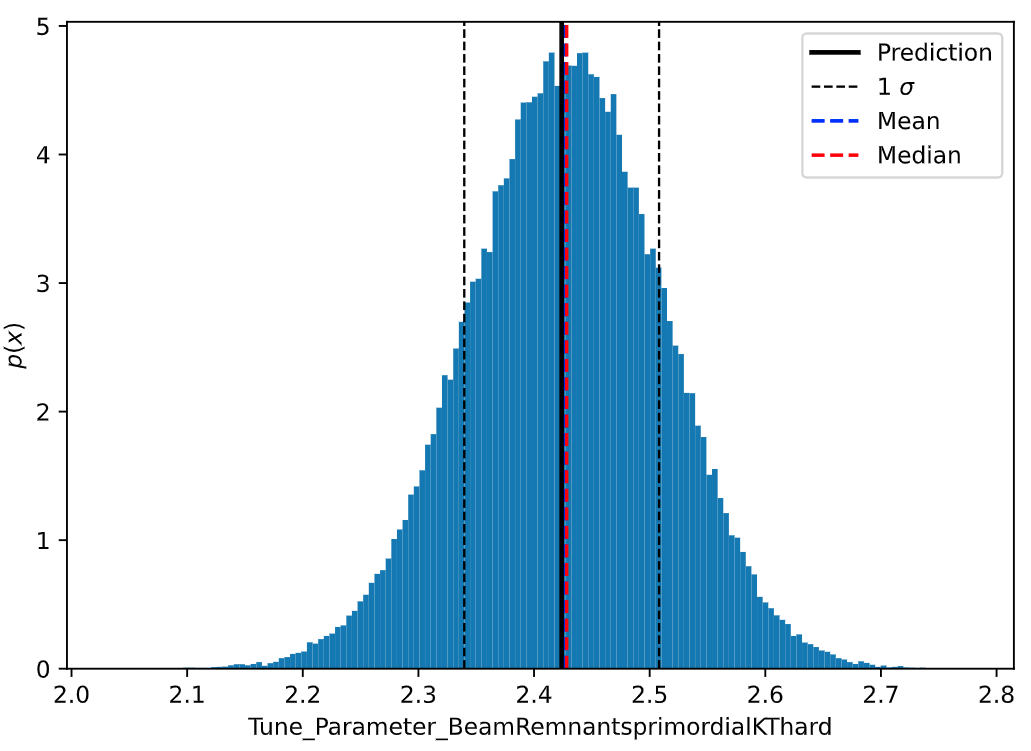
\includegraphics[width=0.6\textwidth]{{img/InverseModel_predictionsSpread.png}}
	\caption{Predictions spread for the inverse model after that a Gaussian resample is performed}
	\label{fig:InverseModel_predictionsSpread}
\end{figure}

Note that this is a new method for the tune. As we are going to see this method requires more attention than the PerBin Model to get it working correctly in the case of a high number of parameters to tune.
\\
With respect to the PerBin Model this method is faster in the training step. The NN trained is only one and is not needed a minimization  so a scan in the hyperparameters can be performed in order to search for the best architecture. 

 
\subsubsection{Hyperparameters}

A really important step in the Inverse model is \textit{hyperparameter optimization}. It is required to get the method working. 

The procedure consists in building a \textit{validation set } containing some Monte Carlo simulations as the training set (e.g. $10\%$ of the simulations in the training set) and retrain the model with different choices for the NN architecture. Then a closure test is performed in order to estimate the performance of the NN. The test is performed using these validation set MC runs as input instead of the real experimental data, the closure test is done by computing a loss function between the predicted value and the Monte Carlo truth defined as:
\begin{equation}
	L=\displaystyle\sum_i \frac{\big|p_i^{\text{true}} - p_i^{\text{pred}} \big|}{p_i^{\text{true}}}
\end{equation} 
\\
The configuration that minimizes the distance between predicted and real values (MC truth), and so this loss function, is the best architecture in the selected hyperparameter space.  
\\
Once the best model is found, it is retrained using the MC runs contained in both the  training and validation sets. Then the experimental data are fed to it in order to get the best estimation for the parameters to tune. This procedure is schematically summarized in \figRef{fig:HyperParams}.
\\
The hyperparameters scan is performed using the python package \texttt{hyperopt}.


\begin{figure}[!htb]
	\centering
	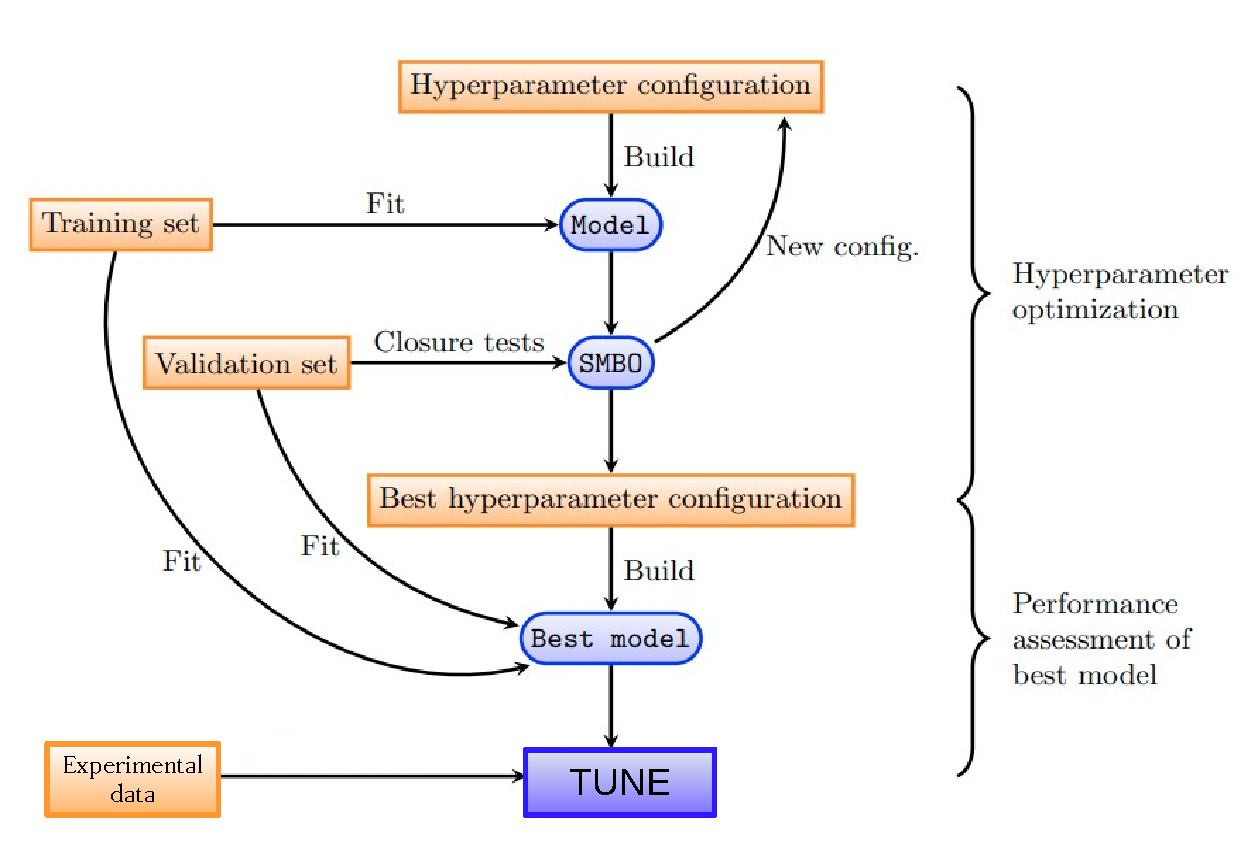
\includegraphics[width=0.9\textwidth]{{img/workflow.pdf}}
	\caption{The hyperparameter optimization procedure is schematically shown here. The model is trained using a training set then performing a closure test a scan on the hyperparameter is done. Once the best configuration is found the best model is retrained using both the runs in the training set and the runs in the validation set. Then the experimental data are fed to the network and the best parameters are estimated. Figure from \cite{MCNNTUNESarticle}}.
	\label{fig:HyperParams}
\end{figure} 

\subsubsection{Problems}

As shown in the next chapter the main problem for the Inverse model is the instability of the results in some cases. The operation that this model is trying to do is very hard the parameters can have some not trivial correlations. This complication can increase a lot the complexity in the operation of learning the inverse response of the generator. These difficulties in some cases lead to a bad prediction with parameters value predicted out of the imposed ranges and with errors in the order of the parameter value. 
\\
As it will be seen in the chapter that describes the new tune performed using the Inverse model in some cases when the number of parameters became larger and maybe the correlation between the parameters are important this model fails in the prediction. 
\\
But if more care is given to this model this can become a very powerful method for future tunes.


\subsection{Weightrules in MCNNTUNES}

\textsc{mcnntunes} as \textsc{professor} implements the possibility of changing the weight of the singles bins in the distributions. This is a really useful feature in order to give some more importance to distributions and points that require a better description by the tune. As it will be discussed later these weightrules can be used  to get results more similar to CP5 in the \textsc{mcnntunes} tune proposed in this thesis. 
This feature gives the possibility to decide which distribution is more important in our tune.
Increasing the weight of a bin this bin became more important in the overall $\chi^2$ evaluation and it is better described by the simulations. 
%An example is shown in \figRef{fig:CMS_weightrules} where the application of the weightrules takes us to a better description of the experimental data.
%
%\begin{figure}[!htb]
%\centering
%\noindent
%	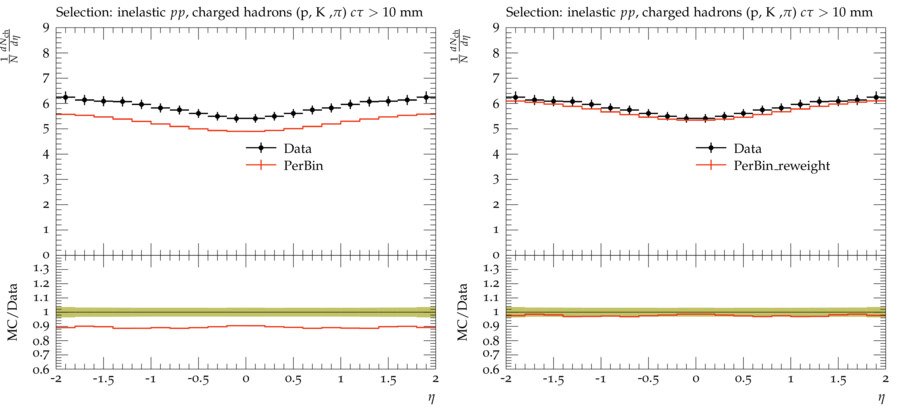
\includegraphics[width=0.85\textwidth]{{img/CMS2015_weightrules.jpg}}
%	\caption{An example of weightrules application. Here the black point are the experimental data from the CMS analysis at $\sqrt{s}=13\ \mathrm{TeV}$ \cite{CMS:2015zrm} while the colored lines are the simulations, the vertical lines on MC points indicate the statistical uncertainties. It is easy to see that the distribution in the right panel is not well described from the tune, but thanks to the weightrules we can give to this distribution a greater importance in the tune and describes it better as shown in the left panel. This is better explained in the next chapter.}
%	\label{fig:CMS_weightrules}
%\end{figure}   


